
\appendix



\subsection{Ridge vs. OLS estimator}
When $\mathbf{X}$ is orthonormal then $\mathbf{X}^\intercal \mathbf{X} =\mathbb{I}$ and there is a simple relation between the ridge estimator and the OLS estimator:

\begin{eqnarray*}
\phi_* (\lambda) &=& (\mathbf{X}^\intercal \mathbf{X}+\lambda \mathbb{I})^{-1}\mathbf{X}^\intercal \mathbf{Y} \\
 &=& (\mathbb{I} + \lambda \mathbb{I})^{-1} \mathbf{X}^\intercal \mathbf{Y} \\
 &=&(1+\lambda)^{-1} \mathbb{I} \mathbf{X}^\intercal \mathbf{Y} \\
 &=&(1+\lambda)^{-1} (\mathbf{X}^\intercal \mathbf{X})^{-1}\mathbf{X}^\intercal \mathbf{Y} \\
 &=&(1+\lambda)^{-1} \phi
\end{eqnarray*}




%\subsection{Geometric interpretation}
%\begin{figure}
%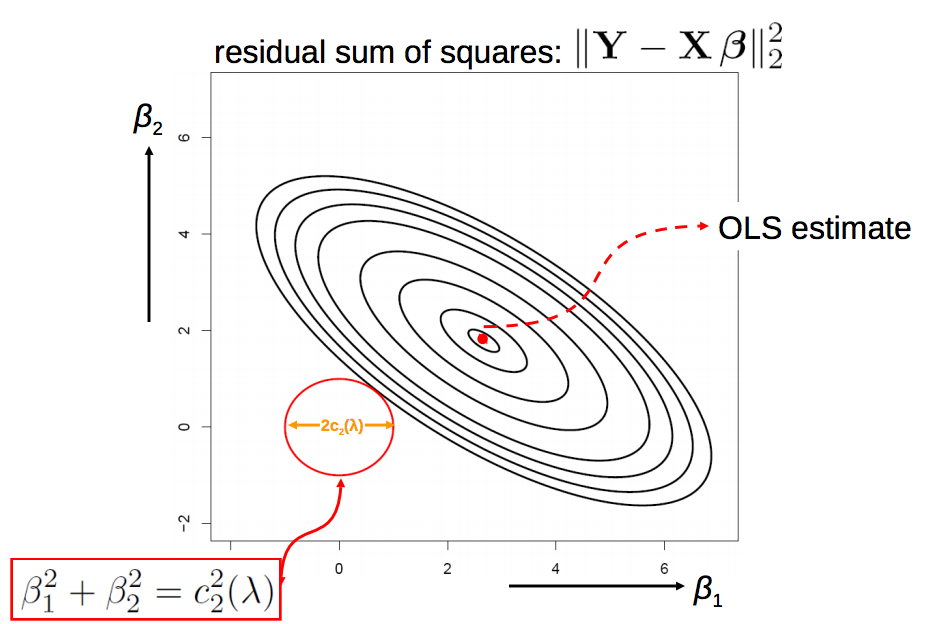
\includegraphics[width=0.9\linewidth]{img/geo1}
%\end{figure}
%\begin{figure}
%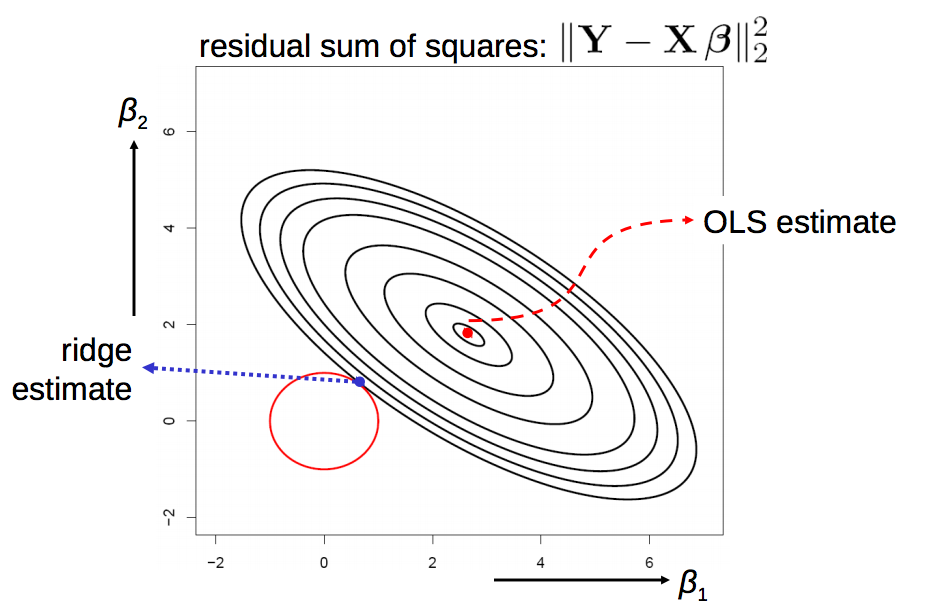
\includegraphics[width=0.9\linewidth]{img/geo2}
%\end{figure}






\section{Sherman Morrison formula} \label{sec:sherman}

Sherman Morrison formula states if a matrix $\mathbf{A}$ is a positive
definite matrix and its inverse matrix is known, then the inverse of the
matrix $\mathbf{B}=\mathbf{A} + \mathbf{x}\mathbf{x}^\intercal$ can be
obtained as: 

\begin{equation*}
\mathbf{B}^{-1} = \mathbf{A}^{-1} -
\frac{(\mathbf{A}^{-1}\mathbf{x})(\mathbf{A}^{-1}\mathbf{x})^{\intercal}}
{1 + \mathbf{x}^{\intercal} \mathbf{A}^{-1} \mathbf{x}} \, .
\end{equation*}

This formula reduces the inverse matrix computation order from $O(n^3)$ to
$O(n^2)$.
